\section{Prototype}

O padrão Prototype permite reduzir a quantidade 
de subclasses definidas em uma aplicação 
substituindo-as por instâncias predefinidas 
que podem ser reutilizadas em tempo de 
execução. Objetos que funcionam como 
protótipos podem ser clonados e assim 
reutilizados por outros objetos, sendo uma 
alternativa à herança. \cite{gamma:1995}

A estrutura do padrão, apresentada na imagem 
\ref{prototype_struct}, mostra uma interface 
Prototype que define a operação Clone, responsável 
por copiar o protótipo reutilizável de um objeto. 
As classes ConcretePrototype implementam essa 
interface e a operação que retorna a cópia. 
A classe Client acessa o protótipo através da operação 
Clone. Essa dinâmica permite que a classe cliente 
não precise conhecer o objeto clonado nem sua 
implementação, o que as torna independentes e 
diminui o acoplamento.

\begin{figure}[htb]
	\caption{\label{prototype_struct}Estrutura do Prototype}
	\begin{center}
	    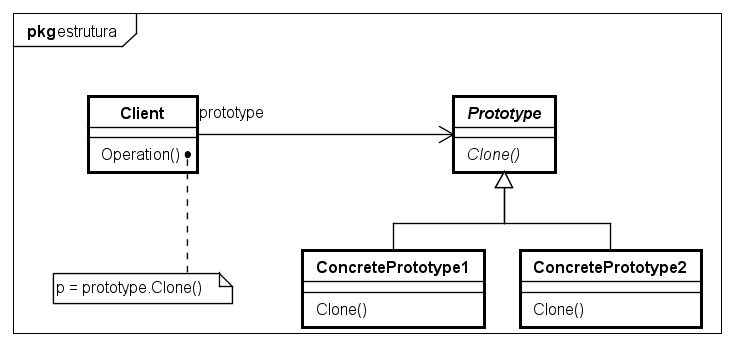
\includegraphics[scale=0.5]{5_padroes-contexto-funcional/5.1_criacionais/5.1.4_prototype/prototype_estrutura.png}
	\end{center}
\end{figure}


\subsection*{Exemplo Orientado a Objetos}

Como exemplo de uso do Prototype, um 
\textit{framework} de editores gráficos deseja 
ser utilizado para construir um editor de 
partituras musicais. A classe responsável pelo 
desenho de elementos gráficos na tela não 
conhece as classes que definem as notas musicais que 
precisam ser desenhadas. Ao invés de criar uma 
subclasse para cada novo elemento gráfico, 
a classe responsável pelo desenho 
pode receber um objeto protótipo qualquer. 
Dessa forma, trocando a herança 
por uma delegação, é possível desenhar qualquer 
elemento musical, desde que ele possa ser 
clonado. A figura \ref{prototype_exemplo} e 
o código \ref{ooprototype} ilustram esse cenário.

\begin{figure}[htb]
	\caption{\label{prototype_exemplo}Exemplo de Prototype}
	\begin{center}
	    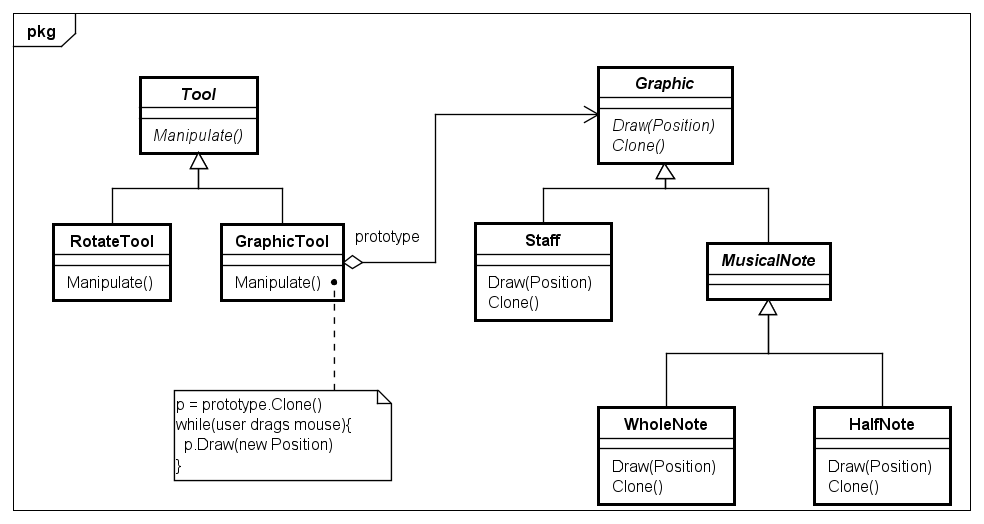
\includegraphics[scale=0.5]{5_padroes-contexto-funcional/5.1_criacionais/5.1.4_prototype/prototype_exemplo.png}
	\end{center}
\end{figure}

\begin{lstlisting}[caption={Prototype Orientado a Objetos},label=ooprototype]

trait Graphic {
  def Draw(position : Position)
  def Clone() : Graphic
}

class Staff extends Graphic {
  def Draw(position : Position) :Unit = {
    println("Desenha elemento")
  }

  def Clone() : Graphic = this.Clone()
}

trait MusicalNote extends Graphic

class WholeNote extends MusicalNote {
  def Draw(position : Position) : Unit = {
    println("Desenha nota musical")
  }

  def Clone() : Graphic = this.Clone()
}

class HalfNote extends MusicalNote {
  def Draw(position: Position): Unit = {
    println("Desenha nota musical")
  }

  def Clone() : Graphic = this.Clone()
}

class GraphicTool(var prototype : Graphic) {

  def Manipulate() : Unit = {
    var p = this.prototype.Clone()
    while(User.DragsMouse()) {
      p.Draw(newPosition)
    }
    //...
  }
}

\end{lstlisting}

\subsection*{Contexto Funcional}

O padrão Prototype fornece uma operação de 
clonagem para que o estado de um objeto seja 
copiado sem ser compartilhado entre todos 
os objetos que o utilizam. Graças ao conceito 
de imutabilidade presente na programação 
funcional, valores definidos podem 
ser reutilizados sem que haja preocupação 
quanto a alterações de seu estado.

O código \ref{fpprototype} demonstra como o 
exemplo orientado a objetos anterior poderia 
ser implementado. A função DrawPrototype, 
definida na linha 2, recebe como parâmetro um 
valor do tipo Graphic - sem preocupar-se se 
esse valor está sendo clonado, reutilizado ou 
se existem mais referências para ele em outras 
funções da aplicação. Ela retorna uma função 
responsável por desenhar esse elemento. Dessa 
forma, a função ManipulateGraphic, na linha 
7, pode apenas receber como parâmetro uma função 
que desenha um elemento gráfico, que pode ser 
alterada dinamicamente de acordo com o elemento 
gráfico desejado.

\begin{lstlisting}[caption={Prototype Funcional},label=fpprototype]
    
def DrawPrototype(graphic: Graphic) : Position => Unit =
  (newPosition : Position) => {
    // Desenha elemento gráfico
  }

def ManipulateGraphic(Draw : Position => Graphic) : Unit = {
  while(dragsMouse){
    Draw(newPosition)
  }
}
    
\end{lstlisting}